\documentclass[a4paper, 6pt, landscape]{scrartcl}
\usepackage[german]{babel}
\usepackage[utf8]{inputenc}
\usepackage{geometry}
\usepackage{multicol}
\usepackage[dvipsnames]{xcolor}
\usepackage{graphicx}
\usepackage{wrapfig}
\usepackage{enumitem}
\usepackage{fancyhdr}
\usepackage{index}
\usepackage{mwe}
\usepackage{comment}
\usepackage{lipsum}
\usepackage{amsmath}
\usepackage{amssymb}
\usepackage{listings}
%Define Math Commands:
\newcommand*{\field}[1]{\mathbb{#1}}%
\newcommand{\Mod}[1]{\ (\mathrm{mod}\ #1)}

%Image Folder:
\graphicspath{{../img/}}

%format
\geometry{top=0.4cm,left=0.5cm,right=0.5cm,bottom=0.4cm}
\setlist{topsep=0pt, leftmargin=5mm, nolistsep}

% Code Snippets

\definecolor{javared}{rgb}{0.6,0,0} % for strings
\definecolor{lightgray}{rgb}{.9,.9,.9}
\definecolor{darkgray}{rgb}{.4,.4,.4}
% define color
\definecolor{sectionColor}{HTML}{7cbad4}
\definecolor{subSectionColor}{HTML}{c7e5b6}
\definecolor{subSubSectionColor}{HTML}{ffeca9}
\definecolor{royalBlue}{HTML}{4A1FBF}
\definecolor{midnightBlue}{HTML}{191970}
\definecolor{codeBackground}{RGB}{245,245,245}
\definecolor{gray}{rgb}{0.5,0.5,0.5}
\definecolor{darkGreen}{RGB}{0,150,0}
\definecolor{DarkPurple}{rgb}{0.4, 0.1, 0.4}

\lstdefinestyle{sharpc}{language=[Sharp]C}
\lstdefinelanguage{JavaScript}{
keywords={const, typeof, new, true, false, catch, function, return, null, catch, switch, var, if, in, while, do, else, case, break},
ndkeywords={class, export, boolean, throw, implements, import, this},
ndkeywordstyle=\color{darkgray}\bfseries,
identifierstyle=\color{black},
sensitive=false,
comment=[l]{//},
morestring=[b]',
morestring=[b]"
}

\lstset{
language=JavaScript,
basicstyle=\fontsize{6}{6} \ttfamily,
keywordstyle=\bfseries\color{royalBlue},
stringstyle=\color{javared},
commentstyle=\color{royalBlue},
morecomment=[s][\color{royalBlue}]{/*}{*/},
tabsize=2,
showspaces=false,
showstringspaces=false,
texcl = true,
rulecolor = \color{black},
backgroundcolor=\color{lightgray},
breaklines = true,
aboveskip = 0em,
belowskip = 0em
}


% Define Section Format
% define section format
\usepackage{sectsty}
\usepackage{titlesec}
\usepackage{graphicx}
\usepackage{graphicx}
\usepackage{graphicx}

\titleformat{name=\section}[block]{\sffamily\small}{}{0pt}{\colorsection}
\titlespacing*{\section}{0pt}{0pt}{0pt}
\newcommand{\colorsection}[1]{%
\colorbox{sectionColor!80}{\parbox{0.98\linewidth}{\vspace{-1pt}\color{black}\ #1 \vspace{-2pt}}}}

% Define Subsection Format
\titleformat{name=\subsection}[block]{\sffamily\small}{}{0pt}{\colorsubsection}
\titlespacing*{\subsection}{0pt}{0pt}{0pt}
\newcommand{\colorsubsection}[1]{%
\colorbox{subSectionColor!80}{\parbox{0.98\linewidth}{\vspace{-1pt}\color{black}\ #1 \vspace{-2pt}}}}

% Define SubSubsection Format
\titleformat{name=\subsubsection}[block]{\sffamily\small}{}{0pt}{\colorsubsubsection}
\titlespacing*{\subsubsection}{0pt}{0pt}{0pt}
\newcommand{\colorsubsubsection}[1]{%
\colorbox{subSubSectionColor!60}{\parbox{0.98\linewidth}{\vspace{-1pt}\color{black}\ #1 \vspace{-2pt}}}}

% -----------------------------------------------------------------------
\begin{document}
    \begin{multicols*}{4}
        \setlength{\columnseprule}{0.4pt}
        \footnotesize

        %! Author = Philipp Emmenegger
%! Date = 09/07/2021

\section{Introduction SPA}
\subsection{Browser-based Applications}
\textbf{Benefits:} Platform independent, including mobile,
No software update, no application, easy maintenance, 
Software can be provided as a service (SaaS - pay as you go),
Code separation\\
\textbf{Liabilities:} No data sovereignty (Datenhoheit),
Limited/restricted hardware access,
SEO - Search engines must execute JavaScript,
More complex deployment strategies

\subsection{SPA}
Fits on a single web page, user experience of a desktop application.
All code is retrieved with a single page load or resources are dynamically loaded.
AJAX and HTML5 to create responsive Web apps, without constant page reloads.

\subsubsection{Bundling}
Code delivered over potentially slow networks.
Bundling and minifying the source leads to smaller SPA footprint.
Larger SPAs with many modules need dependency management.
Initial Footprint reduced by loading dependent modules on-demand.

\subsubsection{WebPack as Bundler}
\textbf{Entry:} Start, follows the graph of dependencies to know what to bundle.
\textbf{Output:} Tell webpack where to bundle your application.
\textbf{Loaders:} Transforms these files into modules as they are added to your dependency graph.
\textbf{Plugins:} Perform tasks like bundle optimization, asset management and injection of env variables.
\textbf{Mode:} Enable built-in optimization mechanisms.

\subsection{Routing}
Completely on client-side by JS. 
Navigation behaves as usual.
Browser needs to fake the URL to change and store page state.
\textit{window.history.pushState}.

\subsection{Dependency Injection}
Reduces coupling between consumer and implementation.
Contracts between classes are based on interfaces.
Supports the open/closed principle.
Allows flexible replacement of an implementation.

\subsubsection{Decorators}
Provide a way to add annotations / meta-programming syntax.
Can be attached to a class declaration, method, accessor, property or parameter.
Widely used in Angular.
        %! Author = Philipp Emmenegger
%! Date = 09/07/2021

\section{React}
\begin{itemize}
    \item Library, kein Framework
    \item Um User Interfaces zu bauen
    \item View in MVC
    \item Minimales Featureset
    \item Entwickelt von Facebook
    \item Verwendet für: WhatsApp, Insta, AirBnb, etc.
\end{itemize}
\subsubsection{Prinzipien}
\begin{itemize}
    \item Komplexes Problem aufteilen in einfachere Komponenten
    \item Für eine bessere: Wiederverwendbarkeit, Erweiterbarkeit, Wartbarkeit, Testbarkeit, Aufgabenverteilung
\end{itemize}

\subsection{Entwicklung von UIs}
\begin{itemize}
    \item Beschreibung des UIs
    \item Event-Handling
    \item Aktualisieren der Views
\end{itemize}

\subsection{Komponenten und Elemente}
\begin{itemize}
    \item Funktionen die HTML zurückgeben
    \item Beliebige Komposition von React-Elementen und DOM-Elementen
\end{itemize}
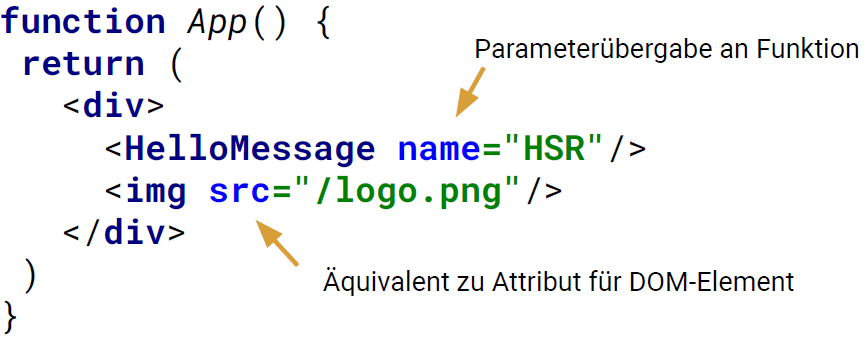
\includegraphics[width=0.6\linewidth]{img/react_component.png}

\subsection{JavaScript XML}
React verwendet JSX (blau), eine Erweiterung von JavaScript (gelb).
Überall wo JSX verwendet wird, muss $react$ importiert werden.\\
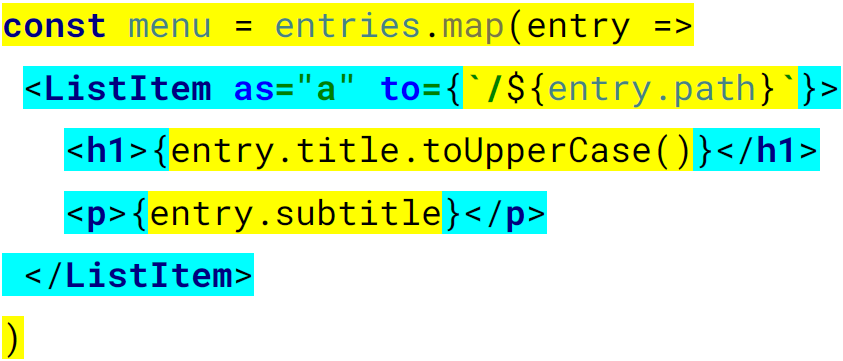
\includegraphics[width=0.6\linewidth]{img/react_jsx.png}\\
\textbf{Styles:} werden nicht als Strings sondern als Object angegeben.

\subsubsection{Conditionals}
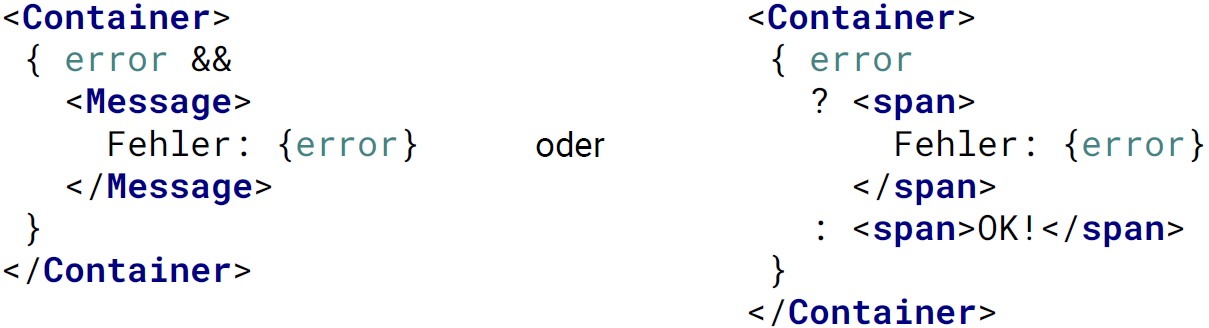
\includegraphics[width=0.7\linewidth]{img/react_jsx_conditionals.png}

\subsubsection{Props}
Komponenten erhalten alle Parameter/Properties als \textbf{props} Objekt.
\begin{itemize}
    \item $this.props$ bei Klassen
    \item Bei Funktionen als Parameter
    \item Immer \textbf{read-only}
\end{itemize}

\subsubsection{Rendering und Mounting}
\textbf{Mounting:} nötig um Komponenten auf Webseite anzuzeigen. \textit{ReactDOM.render}
\begin{lstlisting}
ReactDOM.render(
    <App/>
    document.getElementById('root')
)
\end{lstlisting}

\subsection{React State}
React-Klassenkomponenten können einen veränderbaren Zustand haben.
Der \textbf{state} einer Komponente ist immer privat.
Ändert der State, wird auch die Komponente aktualisiert.
\begin{lstlisting}
class Counter extends React.Component {
    state = { counter: 0 }
    // ...
}
\end{lstlisting}

\subsubsection{Event Handler}
\begin{lstlisting}
const increment = () => {
    this.setState({counter: this.state.counter + 1})
} // ...
<button onClick={this.increment}>
\end{lstlisting}

\subsection{Reconciliation}
\begin{enumerate}
    \item React Komponenten werden als virtueller DOM gerendert
    \item Wird der \textbf{state} geändert, erstellt React einen virtuellen DOM
    \item Alter und neuer DOM werden verglichen
    \item Erst dann werden geänderte DOM-Knoten im Browser erstellt
\end{enumerate}

\subsection{Formulare}
\subsubsection{Input Handling}
\begin{lstlisting}
<form onSubmit={this.handleSubmit}>
<input value={this.state.username}
        onChange={this.handleUsernameChange} //...
</form>
handleUsernameChange = (event) => {
    this.setState({username: event.target.value});
};
handleSubmit = (event) => {
    event.preventDefault();
    //...
}
\end{lstlisting}

\subsection{Komponenten Lifecycle}
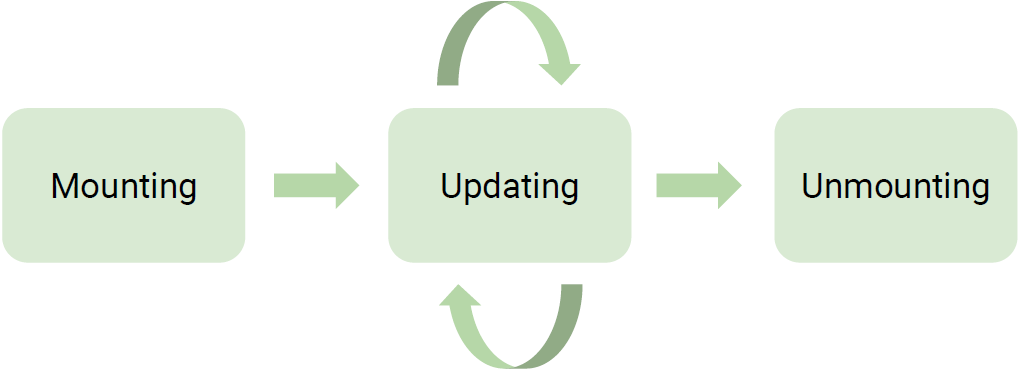
\includegraphics[width=0.7\linewidth]{img/react_lifecycle.png}
\subsubsection{Mounting}
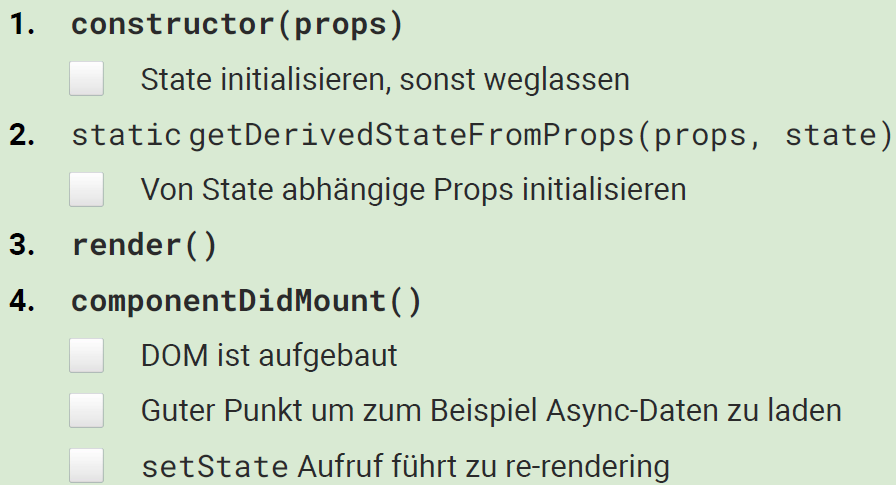
\includegraphics[width=0.7\linewidth]{img/react_mounting.png}

\subsubsection{Updating}
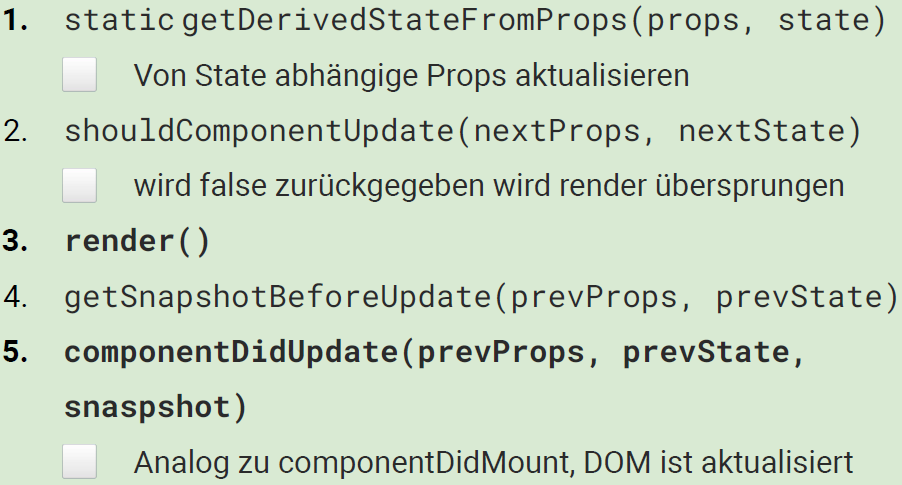
\includegraphics[width=0.7\linewidth]{img/react_updating.png}

\subsubsection{Unmounting}
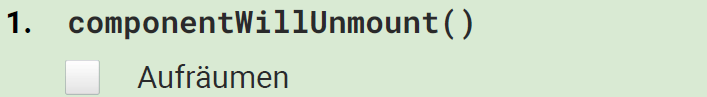
\includegraphics[width=0.6\linewidth]{img/react_unmounting.png}

\subsubsection{Error Handling}
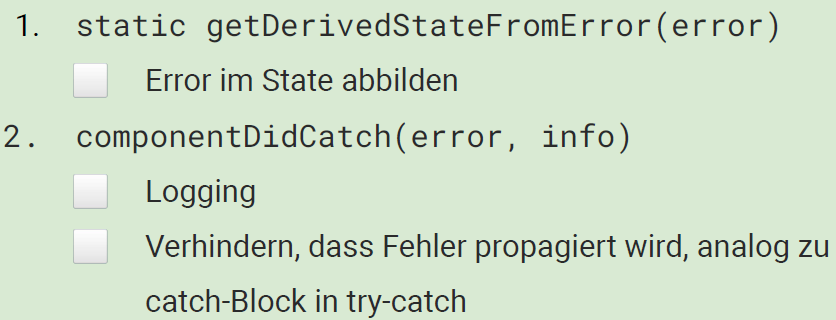
\includegraphics[width=0.7\linewidth]{img/react_error_handling.png}

\subsection{React Router}
\begin{itemize}
    \item Komponentenbibliothek
    \item Komponenten anzeigen oder verstecken abhängig von der URL
    \item Für React Web und React Native
\end{itemize}

\subsubsection{Router Komponenten}
\begin{lstlisting}
<Router>
\end{lstlisting}
Alle Routen müssen Teil des Routers sein, typischerweise nahe der Root-Komponente
\begin{lstlisting}
<Route exact path="/" component={Home} />
\end{lstlisting}
Home-Komponente wird nur gerendert, wenn der path (exakt) matcht.
Mehrere Route Elemente können gleichzeitig aktiv sein.
\begin{lstlisting}
<Link to="/">Home</Link>
\end{lstlisting}
App-interne Links, welche nicht wie \textless a \textgreater die Seite neu laden.
\begin{lstlisting}
<Redirect to="/somewhere/else">
\end{lstlisting}
Wird ausgeführt, sobald gerendert.

\subsection{Hooks}
\textbf{Problem von Lifecycle Methoden}
Zusammengehörender Code ist auf mehrere Methoden verteilt (Mount/Unmount).\\
\textbf{Problem von Klassen-State}
State ist über verschiedene Methoden verteilt\\
\textbf{Fazit:}
\begin{itemize}
    \item Lifecycle und State ohne Klassen machen react verständlicher
    \item Klassen sind weiterhin unterstützt
    \item Hooks erlauben, Logik mit Zustand einfacher wiederzuverwenden
\end{itemize}

\subsubsection{State Hook}
\begin{lstlisting}
function Counter() {
    const [count, setCount] = useState(0);
    // button => setCount(count + 1)
    return( <p>{count}</p> );
}
\end{lstlisting}
\textbf{Mehrere State-Variablen:} useState Aufrufe müssen immer in derselben Reihenfolge gemacht werden.

\subsubsection{Effect Hook}
\begin{lstlisting}
useEffect(() => {
    // Mount stuff
    return () => {
        // Unmount stuff
    }
}, [] /* <= Dependencies */);
\end{lstlisting}

\subsection{Flow}
\begin{itemize}
    \item Erweitert JavaScript um Typenannotationen
    \item Typ-Annotation im Code Typ-Inferenz für lokale Definitionen
    \item Generics, Maybe-Types, Union and Intersection-Types
\end{itemize}

\subsection{TypeScript und React}
\begin{itemize}
    \item Mehr Typensicherheit in React-Komponenten
    \item Props und State lassen sich typisieren
\end{itemize}
\textbf{Vorteil gegenüber Flow:}
\begin{itemize}
    \item Vollwertige Programmiersprache
    \item Besser unterstützt von Libraries und IDEs
    \item TypeScript Fehler müssen korrigiert werden
\end{itemize}

\subsection{React Context}
Ermöglicht es, Props für alle Unterkomponenten zur Verfügung zu stellen. (Theme Variablen)
\begin{lstlisting}
// provider
const c = React.createContext(themes.light);
const theme = useContext(c); // consumer
\end{lstlisting}

\subsection{Redux}
Library für Statemanagement (Repräsentation / Veränderung / Benachrichtigung).
State wird als Tree (immutable) von Objekten dargestellt.
Veränderung am Tree führt durch den Reducer zu einem neuen Tree t+1 (funktionale Programmierung).
State wird im \textbf{Store} verwaltet.

\subsubsection{Actions}
Benötigt um Stateänderungen zu machen.
Wird an den Store gesendet / dispatched.
Action ist eine reine Beschreibung der Action.
\begin{lstlisting}
{type: 'TRANSFER', amount: 100 }
\end{lstlisting}

\subsubsection{Reducer}
Pure Funktionen, haben keine Seiteneffekte.
\begin{lstlisting}
function balance(state = 0, action) {
    switch (action.type) {
        case 'TRANSFER':
            return (state + action.amount);
        default:
            return state;
    }
}
\end{lstlisting}
\textbf{Reducer kombinieren:} Jeder Reducer erhält einen Teil des States, für den er zuständig ist.
Resultat wird in einem neuen State-Objekt kombiniert.
\begin{lstlisting}
function rootReducer(state = {}, action) {
    return {
        balance: balance(state.balance, action),
        transactions: transactions(state.transactions, action)
    }
}
// Hilfsfunktion combineReducers:
const rootReducer = combineReducers({
    balance, transactions
});
\end{lstlisting}

\subsubsection{Store erstellen}
\begin{lstlisting}
const store = createStore(rootReducer);
\end{lstlisting}
Mit dem root-Reducer kann der Store erstellt werden.
In Kombination mit React führt das zu einem re-rendering der Komponenten.

\subsection{React \textless 3 Redux}
\textbf{Redux mit React verbinden:}
\begin{lstlisting}
const mapStateToProps = (state) => {
    return {
        transactions: state.transactions
    }
}
const mapDispatchToProps = {
    fetchTransactions
}
export default connect(mapStateToProps, mapDispatchToProps)(Component);

// Root Komponente
const store = createStore(
    rootReducer, applyMiddleware(thunkMiddleware));
render(
    <Provider store={store}>
        <App />
    </Provider>
    document.getElementById('root')
)
\end{lstlisting}
\textit{mapStateToProps:} erhält State und kann daraus Props ableiten.\\
Die Komponente bekommt auch die \textit{dispatch} Methode des Stores als Prop.
Das Resultat von \textit{connect} ist eine React-Komponente die mit dem Store verbunden ist.\\
Store muss der Root-Komponente mitgegeben werden.\\
\textit{thunkMiddleware:} Erlaubt es, anstelle eines Objektes eine Funktion zu dispatchen (benötigt für asynchrone Actions).

\subsubsection{Thunk Actions}
\begin{lstlisting}
function fetchTransactions(token) {
    return (dispatch, getState) => {
        dispatch({type: "FETCH_TRANSACTIONS_STARTED"});
        api.getTransactions(token)
            .then(({result: transactions}) => {
                dispatch({type: "FETCH_TRANSACTIONS_SUCCEEDED", transactions});
            })
    };
}
\end{lstlisting}

\subsubsection{Selectors}
Getter bei den Reducern, die einen Subtree des Stores zurückgeben.
Wissen über den Aufbau des State-Trees bleibt bei den Reducern.
        %! Author = Philipp Emmenegger
%! Date = 12/07/2021

\section{Firebase}
Läuft in der Google Cloud Platform.
Hauptfokus von Firebase sind Mobile- und Web-Apps.

\subsection{Firebase Authentication}
Backend Services für Authentifizierung und einfache Userverwaltung.
SDKs für diverse Plattformen.
Vorgefertigte UI Libraries

\subsection{Firebase Hosting}
Einfaches Hosting für statischen Content.
\begin{itemize}
    \item Immer per HTTPS ausgeliefert
    \item Automatisches Caching in CDNs
\end{itemize}
Dynamischer Content nur über \textbf{Cloud Function}, wenn das nicht reicht:
\begin{itemize}
    \item PaaS: Google App Engine
    \item Docker: Google Container oder Kubernetes Engine
\end{itemize}

\subsubsection{Serverless Computing}
Cloud Provider verwaltet Functions:
\begin{itemize}
    \item Deployment geschieht on-demand
    \item Plattform bestimmt die Parallelisierung
    \item Entwickler hat keine Kontrolle über laufende Instanzen
    \item Funktionen sind Stateless
    \item Abgerechnet werden Aufrufe und Laufzeit der Funktion
\end{itemize}
\textbf{Limitationen:} Ausführungszeit / Memory begrenzt.
Teilweise hohe Latenz.

\subsubsection{Firebase Cloud Functions}
\textbf{Anwendungszenarien:} Code als Reaktion auf einen Event ausführen,
Administration (Cron Jobs), REST API für Mobile und SPAs zur Verfügung stellen.

\subsubsection{Cloud Firestore}
\begin{itemize}
    \item NoSQL, document-oriented database
    \item DB besteht aus mehreren Collections mit Documents
    \item Document ist ein JSON-Objekt
    \item Document kann Collections beinhalten
    \item Vergleichbar mit MongoDB
    \item Stark eingeschränkte Queries (keine Volltextsuche)
\end{itemize}
\begin{lstlisting}
// Auf Collections / Documents zugreifen
const colRef = db.collection("todos");
const docRef = db.collection("todos").doc("...");
// Dokumente erstellen
db.collection("todos").add({text: "..."});
// Dokument bearbeiten
.doc("...").update({text: "..."});
// Daten Abfragen
db.collection("todos").doc("...").get().then(d => {
    if(!doc.exists) { /* ... */ }
    else { console.log(d.data()); }
}).catch(err => { /* ... */ });
// Daten abfragen mit Filter
db.collection("todos").where("checked", "==", true)
    .orderBy("createdAt").get().then(snapshot => {
// ...
});
\end{lstlisting}

\subsubsection{NoSQL One-To-Many}
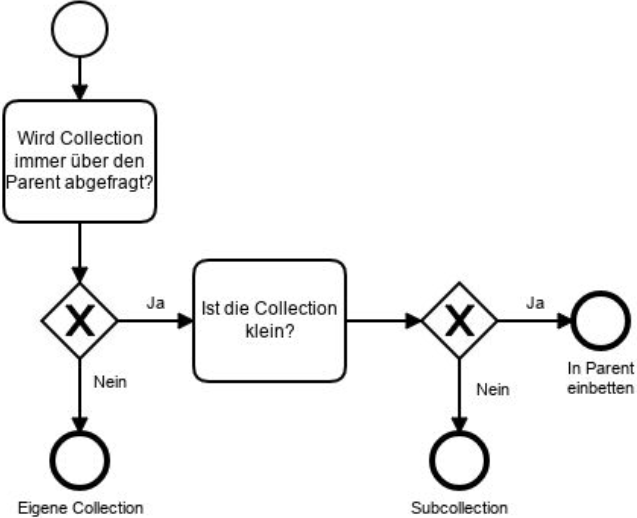
\includegraphics[width=0.6\linewidth]{img/nosql_one_to_many.png}

\subsubsection{NoSQL Many-To-Many}
\begin{itemize}
    \item Wie in relationaler Datenbank mit Assoziationstabelle
    \begin{itemize}
        \item Kein kopieren von Daten
        \item Komplexere Abfragen, keine Joins im Firestore
    \end{itemize}
    \item Oder Daten kopieren und einbetten
\end{itemize}
\textbf{Kopieren der Daten:} muss kein Nachteil sein.
Preisänderung eines Produktes hat keinen Einfluss auf vergangene Bestellungen.
Adressänderung eines Kunden verändert keine alten Bestellungen.
Kopierte Daten können mittels Trigger und Cloud Function wieder synchronisiert werden.
        %! Author = Philipp Emmenegger
%! Date = 12/07/2021

\section{Angular}
Flexible SPA Framework for CRUD applications
\begin{itemize}
    \item Typescript 4.1 based
    \item Reduces boilerplate Code
    \item Dependency Injection Mechanism
    \item JS-optimized 2-way binding
    \item Clearly structured, information hiding
    \item Increases testability / maintainability of client-side code
\end{itemize}


\subsection{Architecture}
\textbf{ngModules:} Cohesive block of code dedicated to closely related set of capabilities. (\textit{module})
\textbf{Directives:} Provides instructions to transform the DOM. (\textit{class})
\textbf{Components:} Directive-with-a-template; it controls a section of the view. (\textit{class})
\textbf{Templates:} Form of HTML defining how to render the component. (\textit{HTML / CSS})
\textbf{Metadata:} Describes a class and defines how to process it. (\textit{decorator})
\textbf{Services:} Provides logic of any value, function or feature that the app needs. (\textit{class})

\subsection{Angular Modules (ngModule)}
Base for Angular modularity system. Every app has at least one Module, the root Module (a.k.a app).
Root Module ist launched to bootstrap the app.
Modules export features (directives, services) required by other modules.\\
\textbf{TypeScript Module vs. ngModule:}\\
ngModule is a logical block of multipe TypeScript modules linked together.
The ngModule declaration itself is placed into a TypeScript module.
Modules can accommodate sub-modules. All public TS members are exported as an overall \textit{barrel}
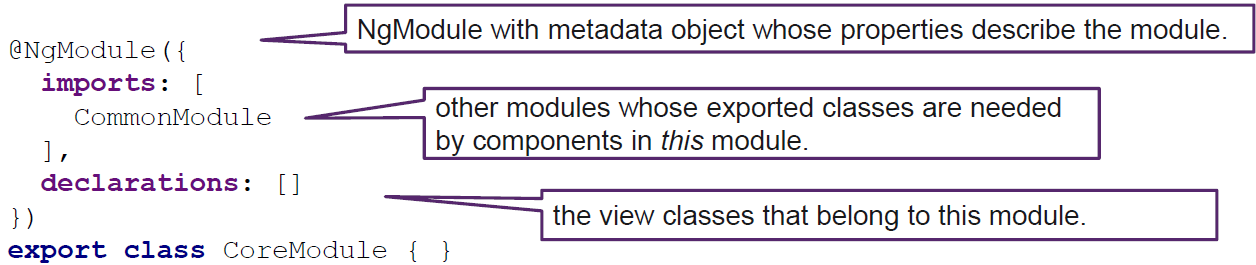
\includegraphics[width=\linewidth]{img/angular_module_declaration.png}
\textit{declarations:} View Classes that belong to this module (Components, Directives, Pipes).\\
\textit{exports:} Subset of declarations that should be visible and usable by other modules.\\
\textit{imports:} Specifies the modules which exports/providers should be imported.
\begin{itemize}
    \item forChild-Import: returns an object with a \textbf{providers} and \textbf{ngModule} property
    \begin{itemize}
        \item allows you to configure services for the current Module level
        \item Use if you need to configure the foreign module
    \end{itemize}
    \item forRoot-Import:  returns an object with a \textbf{providers} and \textbf{ngModule} property
    \begin{itemize}
        \item It provides and condigures services at the same time
        \item Will instantiate the required services exactly once, globally
        \item If no configuration is required, use tree shakable providers \textit{\{ providedIn: 'root'\}}
    \end{itemize}
\end{itemize}
\textit{providers:} Creators of services that this module contributes to the global collection of services (DI Container).
They become accessible in all parts of the app.\\
\textit{bootstrap:} Main application view, root component.
Only the root module should set this property.

\subsubsection{Module Types}
\textbf{Root / App Module:} Provides the entry point (bootstrap component) for the app.
Has no reason to export anything.
\textbf{Feature Modules:} Specifies boundaries between app features.
\begin{itemize}
    \item Domain Modules: Deliver a UI dedicated to a app domain
    \item Routing Modules: Specifies routing configurations
    \item Service Modules: Provides utility services
    \item Widget Modules: Makes components, directives and pipes available to external modules
    \item Lazy Modules: Lazily loaded feature modules
\end{itemize}
\textbf{Shared Modules:} Provides globally used components/directives/pipes.
Is a global UI component module.
Do not specify app-wide singleton providers in a shared module.
\textbf{Core Module:} Keeps your Root Module clean.
Contains components/directives/pipes used by the Root Module.
Globally used services can be declared here.
Only imported by the Root Module


\subsection{Components}
Manages the view and binds data from the model. Consists of:
\begin{itemize}
    \item Controller (App logic), TS Class with \textit{@Component} decorator
    \item HTML file, visual interface (HTML / template expression)
    \item (S)CSS file, styles behind HTML
\end{itemize}
Can be nested, results in Component tree.\\
Provide \textbf{Information Hiding:}
\begin{itemize}
    \item Each Component declares part of the UI
    \item Should be implemented as small coherent piece to support:
    \begin{itemize}
        \item Testability, Maintainability, Reusability
    \end{itemize}
\end{itemize}
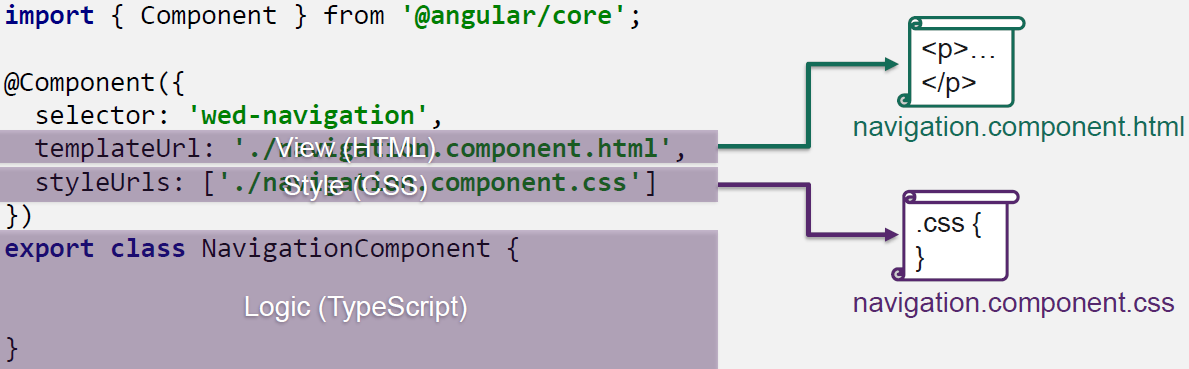
\includegraphics[width=\linewidth]{img/angular_component_declaration.png}
Components must be declared within the containing module so its \textbf{selector} is registered for all sub-components of that module.
They can be exported, so other modules can import and use then.

\subsubsection{Component Lifecycle}
\begingroup
\setlength{\intextsep}{0pt}
\setlength{\columnsep}{20pt}
\begin{wrapfigure}{r}{0.3\linewidth}
    \centering
    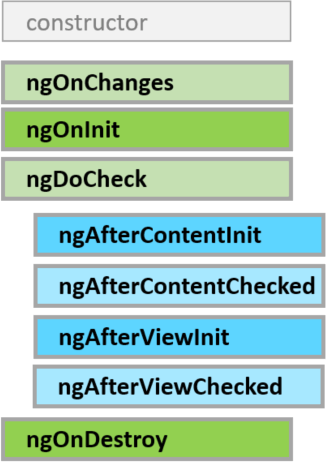
\includegraphics[width=0.7\linewidth]{img/angular_component_lifecycle.png}
\end{wrapfigure}
Most important events are \textbf{ngOnInit} (Creation / Hydration) and \textbf{ngOnDestroy} (Destruction / Dehydration).\\
\textbf{ngAfter...} events are mainly for control developers to handle sub-components and their DOM.
To hook into the lifecycle, interfaces of the Angular core can be implemented.
Each interface has a single hook method, prefixed with \textit{ng}. (\textbf{OnInit} contains method \textit{ngOnInit}).\\
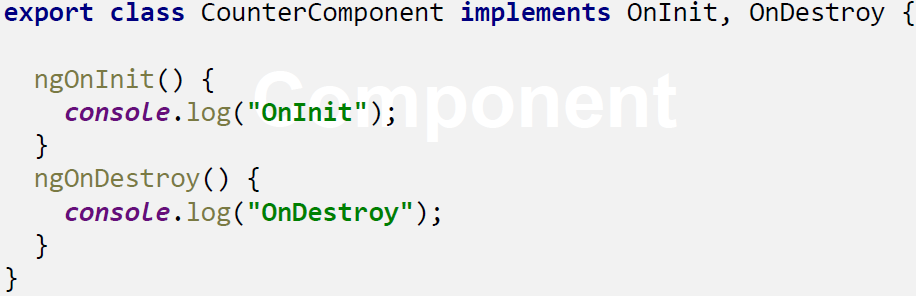
\includegraphics[width=\linewidth]{img/angular_component_lifecycle2.png}

\subsubsection{Content Projection}
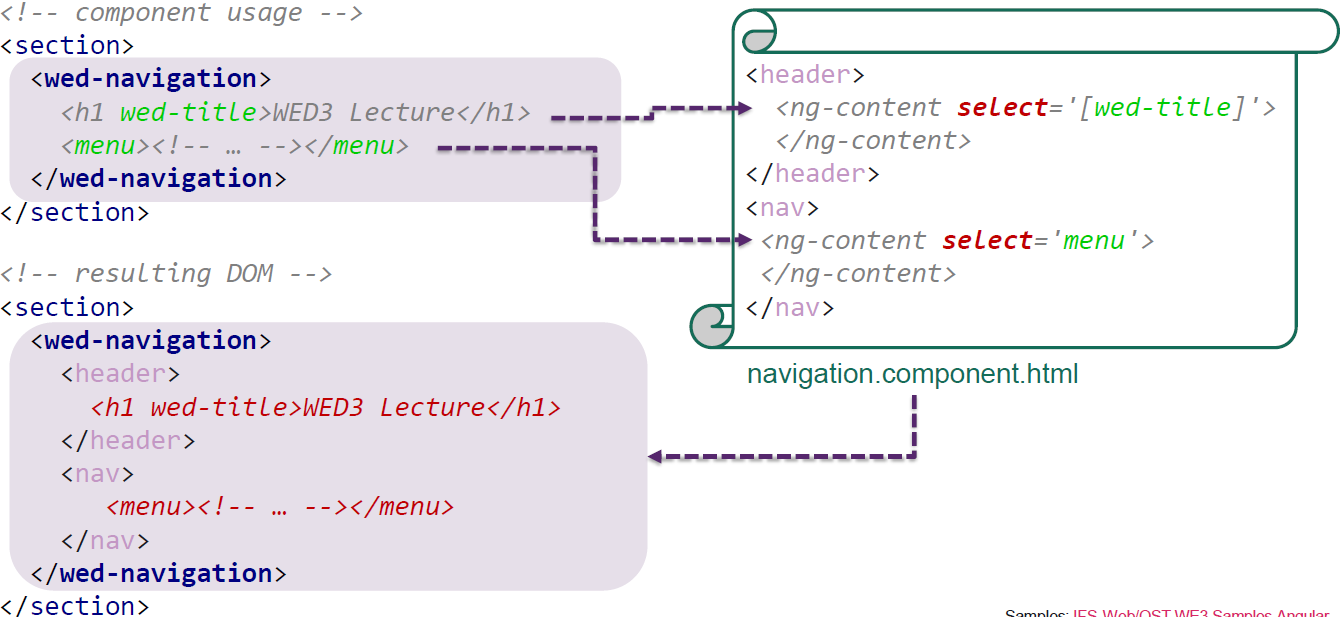
\includegraphics[width=\linewidth]{img/angular_content_projection.png}

\subsection{Templates}
View in MVC.
Written in HTML annotated with Angular \textbf{template syntax}:
\begin{itemize}
    \item HTML5 except script-Tag
    \item Angular extends the HTML with
    \begin{itemize}
        \item Interpolation (\textit{{{...}}})
        \item Template Expression/Statements
        \item Binding Syntax
        \item Directives
        \item Template Reference Variables
        \item Template Expression Operators
    \end{itemize}
\end{itemize}

\subsubsection{Binding}
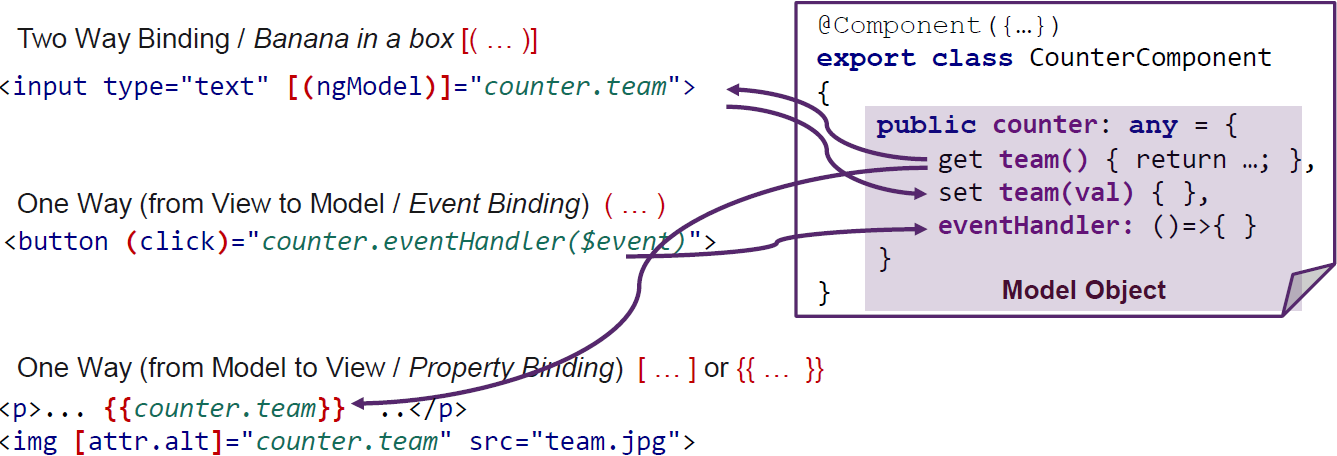
\includegraphics[width=\linewidth]{img/angular_bindings.png}
Binding targets must be declared as \textbf{Inputs or Outputs:} Targets stand on the left side of the binding declaration.
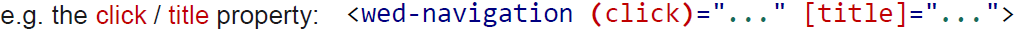
\includegraphics[width=\linewidth]{img/angular_input_output_properties.png}
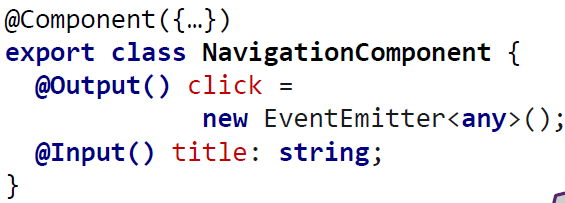
\includegraphics[width=0.5\linewidth]{img/angular_input_output_properties2.png}

\subsection{Directives}
Similar to a component, but without a template.
TypeScript class with an \textit{@Directive()} function decorator.
\subsubsection{Attribute Directives}
Changes the appearance or behaviour of an element, component or another directive.
Applied to a host element as an attribute.
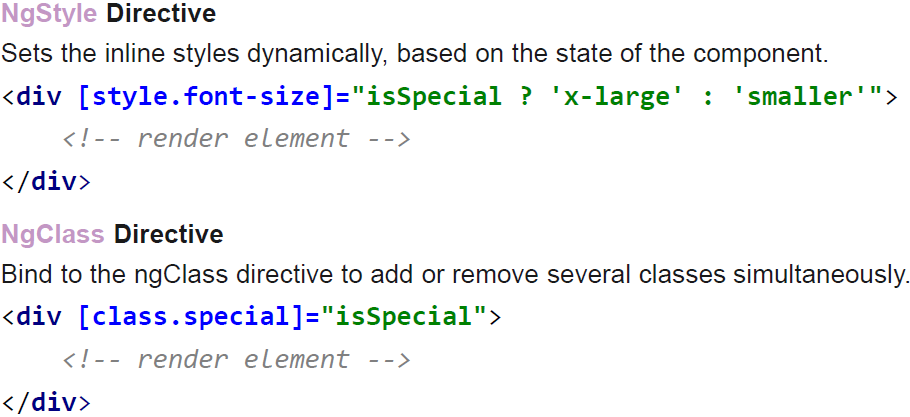
\includegraphics[width=0.6\linewidth]{img/angular_attribute_directives.png}
\subsubsection{Structural Directives}
Responsible for HTML layout.
Reshape the DOM's structure by adding, removing or manipulating elements.
Applied to a host element as an attribute.
Asterisk (*) precedes the directive attribute name.\\
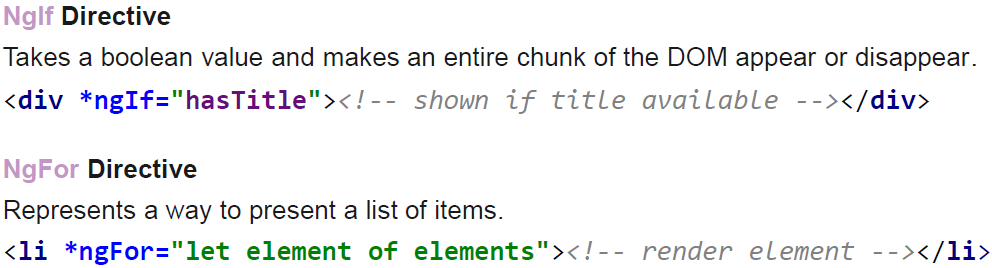
\includegraphics[width=0.7\linewidth]{img/angular_structural_directive.png}\\
\textbf{NgTemplates:}\\

\includegraphics[width=0.8\linewidth]{img/angular_ng_templates.png}\\
Aren't rendered directly.
They need a directive or component which takes over this part.
Can be referenced by their \textit{\#id}:\\
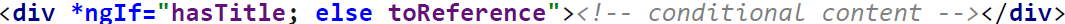
\includegraphics[width=0.8\linewidth]{img/angular_ng_templates2.png}

\subsubsection{Template Reference Variables}
References a DOM element within a template.
Can also be a reference to an component or directive.
A hash (\#) declares a reference variable.\\
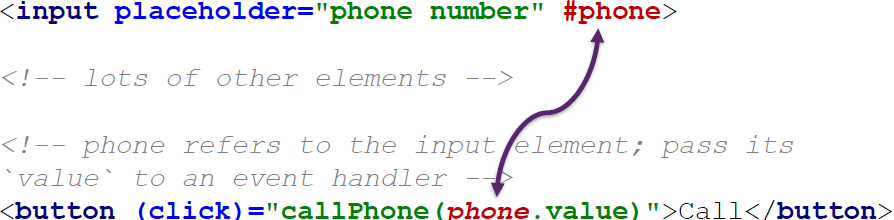
\includegraphics[width=0.7\linewidth]{img/angular_template_reference.png}


\subsection{Services}
Provides any value, function or feature.
Typical Services: logging service, data service, message bus, tax calculator, etc.\\
\textbf{Strongly related to DI:} Angular uses DI to provide components with needed services.
Therefore, services must be registered within the DI container.
\begin{lstlisting}
@Injectable ({ providedIn: 'root' })
export class CounterService { /* ... */ }
\end{lstlisting}
\textit{providedIn: 'root'}: The service is registered for the whole application.
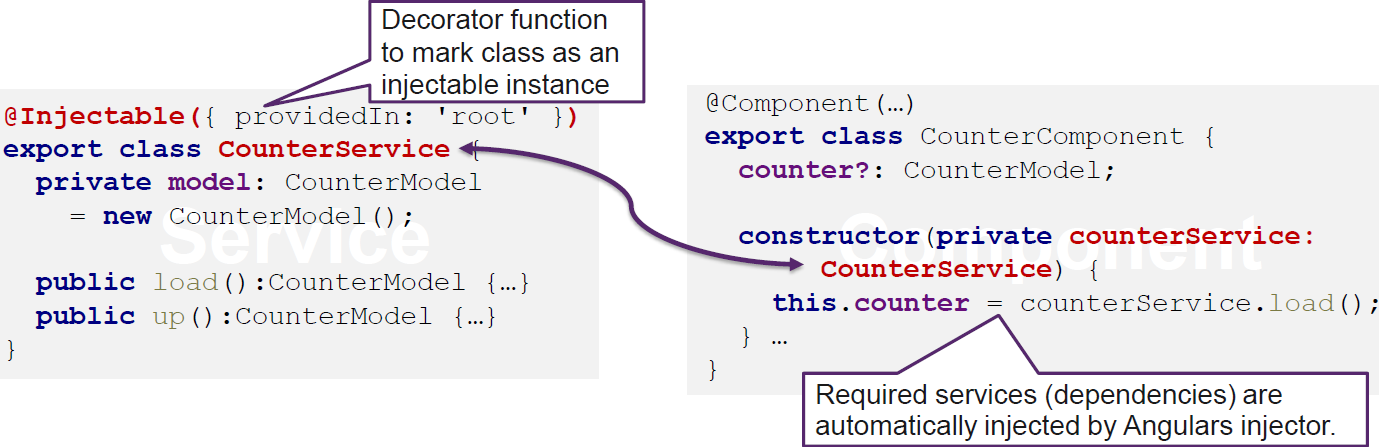
\includegraphics[width=\linewidth]{img/angular_services.png}


\subsection{Forms}
Angular Forms is an external, optional ngModule called FormsModule.
It's a combination of multiple provided services and multiple directives (ngModel, ngForm, ngSubmit).\\
\textbf{Template-driven forms:} Angular Template syntax with the form-specific directives and techniques.
Less code but places validation logic into HTML. (Useful for small forms)\\
\textbf{Reactive / model driven forms:} Import ReactiveFormsModule.
Form is built within the Controller (FormBuilder).
Validation logic is also part of the controller (easier to test).

\subsubsection{Template-driven}
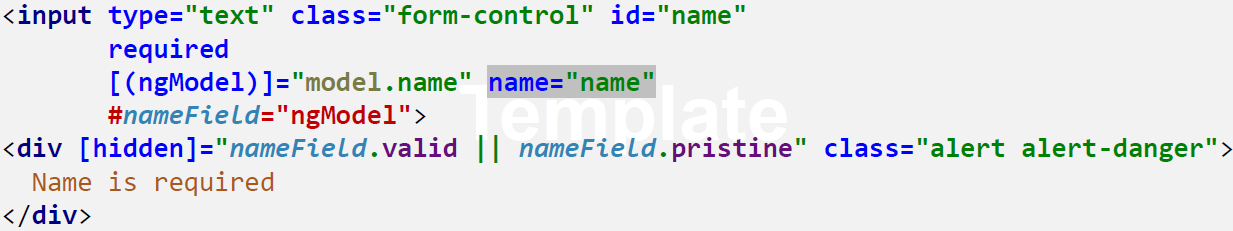
\includegraphics[width=\linewidth]{img/angular_forms.png}
\textbf{Two-Way-Binding:} [(ngModel)] directive to bind values.
Reads out the value of the model for the first time.
Updates are automatically written back into the bound model.\\
\textbf{Validation:} Reference the [ngModel] directive and check its valid property.\\
\textbf{Submitting the form:}\\
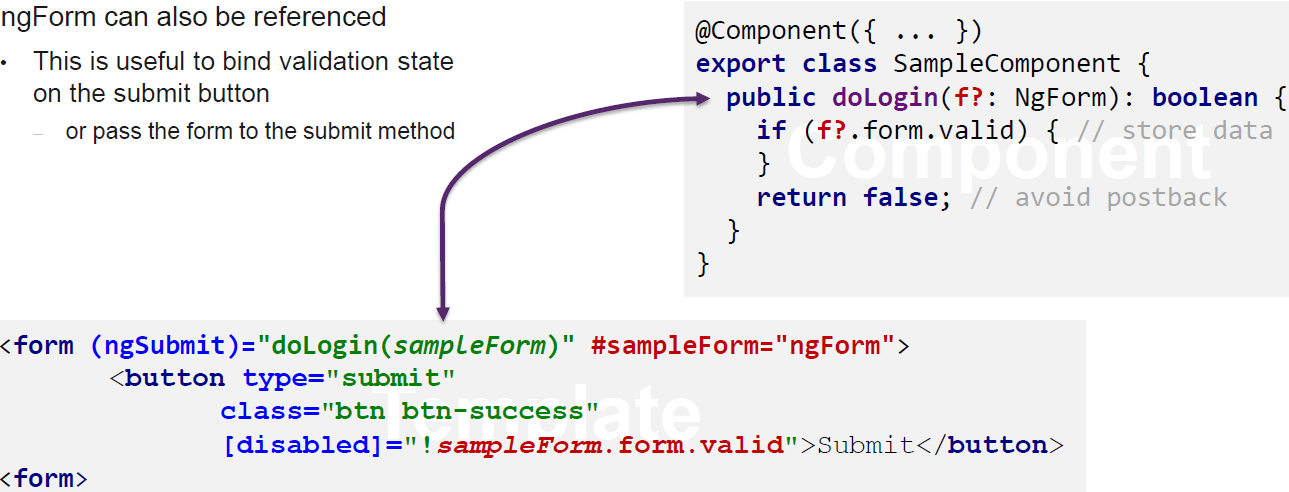
\includegraphics[width=0.8\linewidth]{img/angular_forms_submit.png}


\subsection{Asynchronous Services}
\textbf{Event Emitter example:}\\
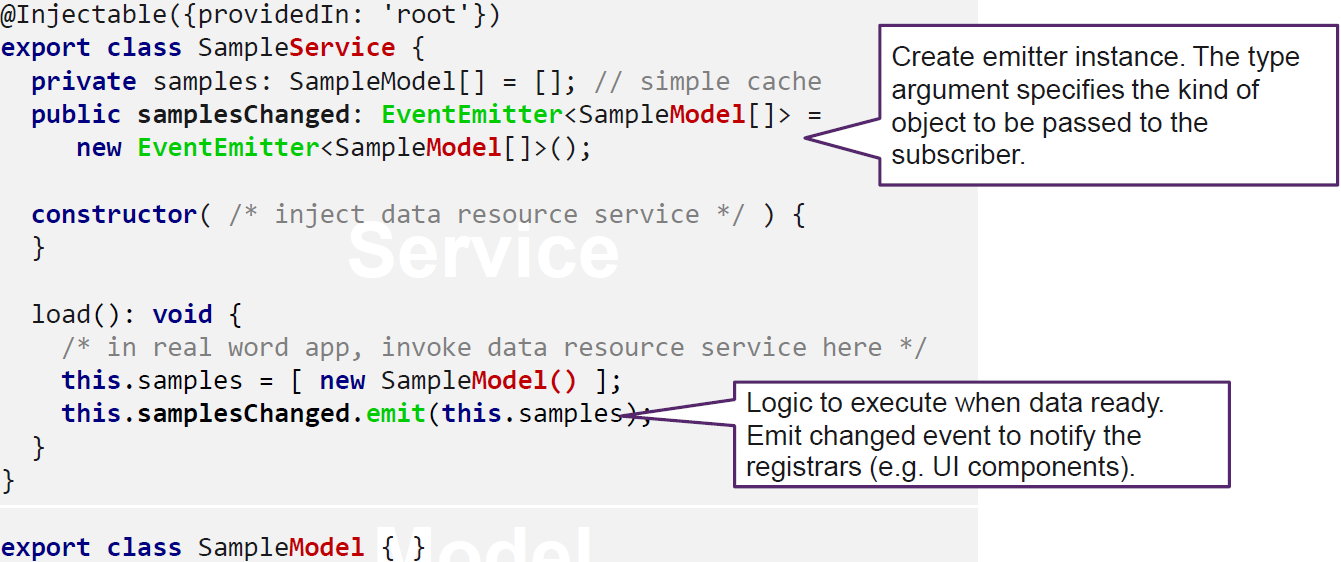
\includegraphics[width=\linewidth]{img/angular_asynchronous_services.png}
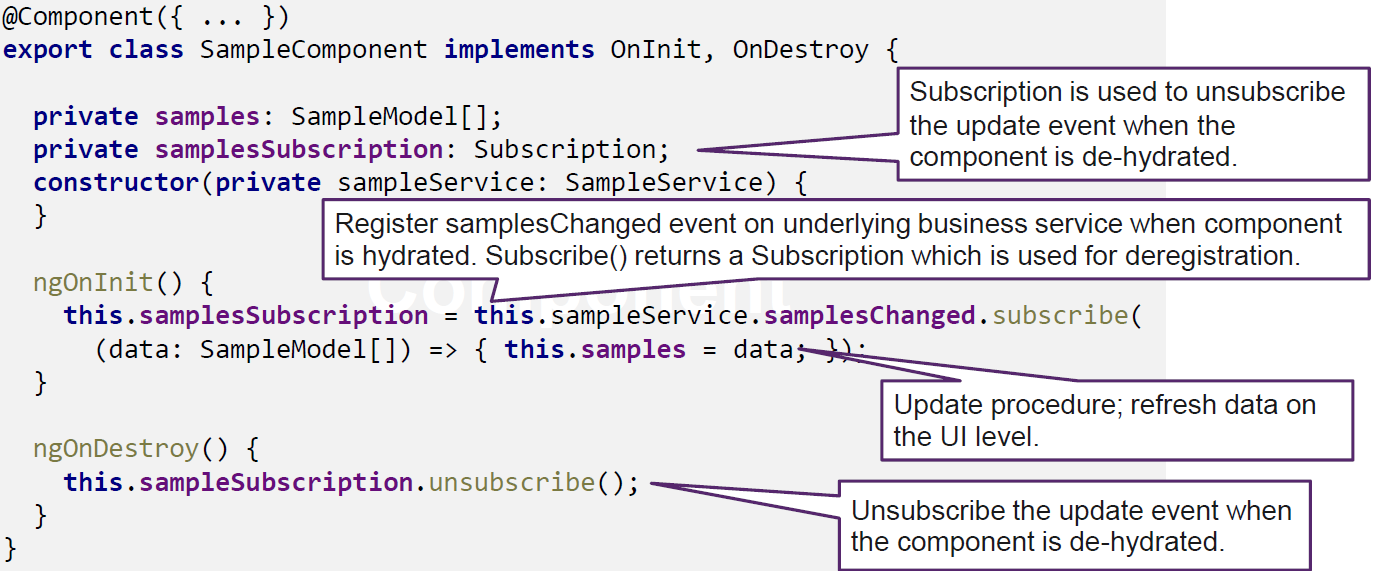
\includegraphics[width=\linewidth]{img/angular_asynchronous_services2.png}

\subsection{Data Access}
\subsubsection{HTTP Client API}
Implements asynchronisms by using the RxJS library.
RxJS is a third-party library that implements the Observable pattern.
An Observable can be turned into a promise.\\
\textbf{Hot Observables:} Sequences of events (mouse moves / stock tickers).
Shared amoung all subscribers.
Postfix hot-observables with a \$\\
\textbf{Cold Observables:} Start running on subscriptions (such as async web requests).
Not shared amoung subscribers.
Are automatically closed after Task is finished.\\
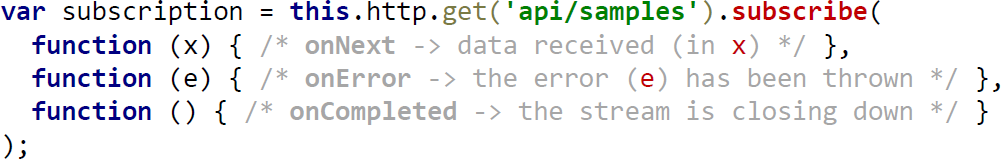
\includegraphics[width=0.8\linewidth]{img/angular_observable.png}


\subsection{Routing}
External, optional NgModule called RouterModule.
Combination of multiple provided services and directives: \textit{RouterOutlet, RouterLink, RouterLinkActive}.\\
\textbf{Defining Routes:} The router must be configured with a list of route definitions.
Each definition maps a route to a component.
\begin{itemize}
    \item \textit{.forRoot():} use exactly once to declare routes on root level
    \begin{itemize}
        \item contains all the directives, the given routes and the router service itself
        \item Every app has one singleton instance of the router
    \end{itemize}
    \item \textit{.forChild():} When declaring sub-routings
    \begin{itemize}
        \item contains all directives and the given routes
    \end{itemize}
\end{itemize}
Each ngModule defines its own routes.
Load modules on-demand (lazy load) with the \textit{import}-Syntax.\\
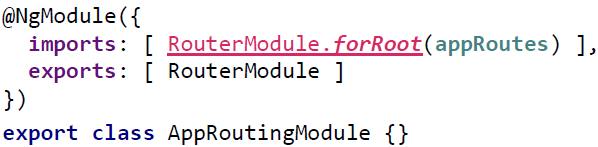
\includegraphics[width=0.5\linewidth]{img/angular_routing.png}
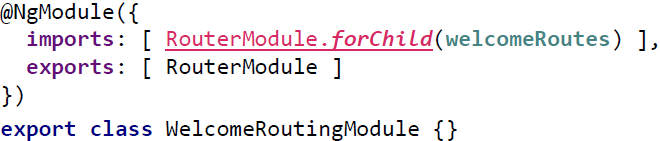
\includegraphics[width=0.5\linewidth]{img/angular_routing2.png}
\textbf{Router Outlet:} Directive from the Router module.
Defines where the Router should display the views.
\begin{lstlisting}
<router-outlet></router-outlet>
\end{lstlisting}
\textbf{Route Configuration:}
\begin{lstlisting}
const appRoutes: Routes = [
    // matches /hero/42, 42 saved in param
    {path: 'hero/:id', component: 'Hero'},
    // redirect
    {path: '', redirectTo: '/heroes', pathMatch: 'full'},
    // Wildcard route
    {path: '**', component: PageNotFound}  
];
\end{lstlisting}
The router uses a first-match-wins strategy.\\
\textbf{Lazy Loading Configuration}\\
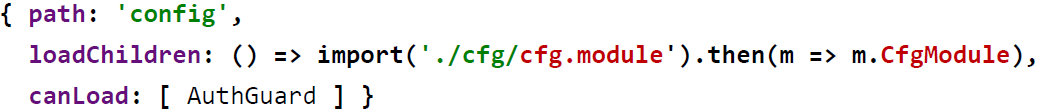
\includegraphics[width=0.8\linewidth]{img/angular_lazy_loading_routes.png}


\subsection{Angular Architectures}
\subsubsection{MVC+S}
\textbf{Observable Business Data Service:} Provides data to multiple parts of the app in a stream-like manner.
An \textit{Observable} is provided.
Stores/Caches business objects.\\
\textbf{RxJS Subject:} Heart of an observable data service. \textit{EventEmitter<T>} derives from Subject.
Hot Observable and does not provide the latest value.\\
\textbf{Behaviour Subject:} Emits the initial state.
Can be called some kind of warm.
Stores the data and emits \textit{next()} events on change.
Do not expose to the Service API.\\
\textbf{Data Resources:} Return cold Observables.
Must be converted into a hot Observable (\textit{share()}).\\
\textbf{Observable Business Data Service Example:}
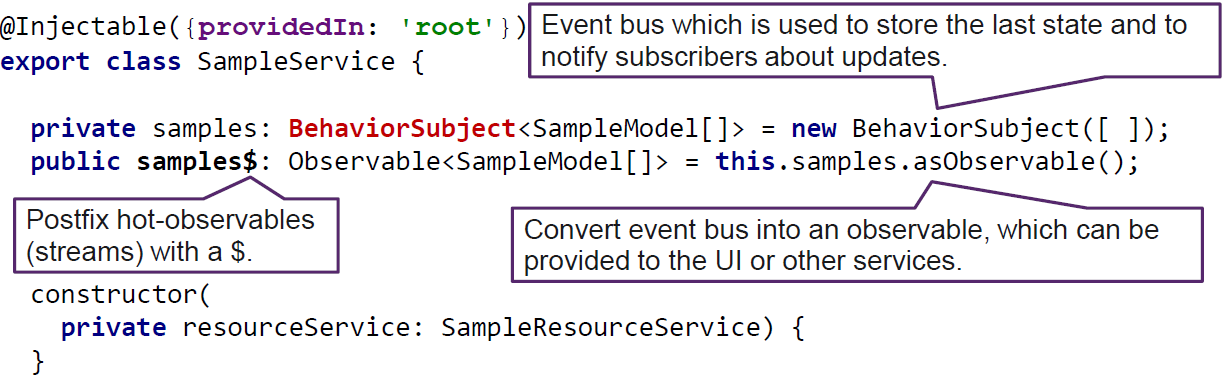
\includegraphics[width=\linewidth]{img/angular_observable_business_data_service.png}
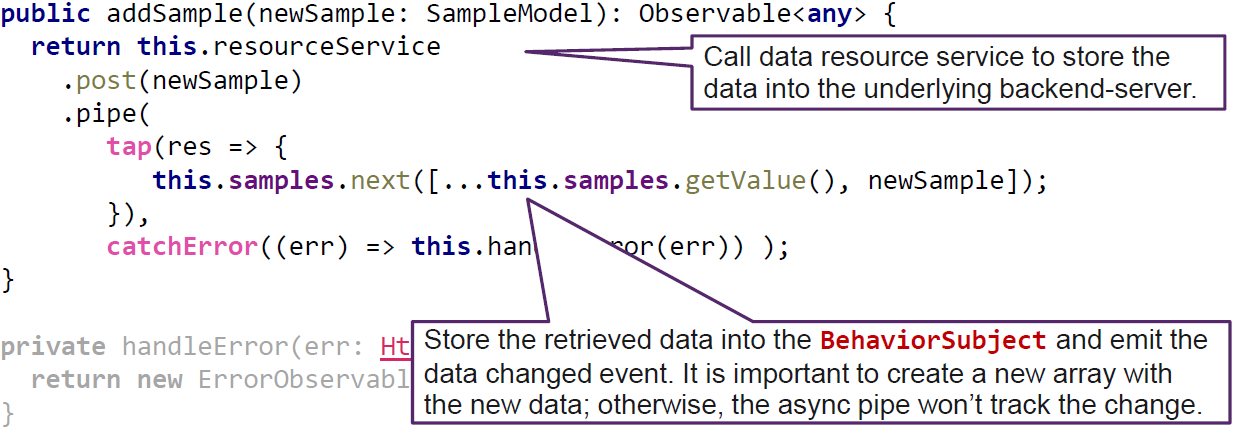
\includegraphics[width=\linewidth]{img/angular_observable_business_data_service2.png}

\subsubsection{Flux Architecture}
Invented by Facebook.
Enforces a unidirectional data flow.
More of a pattern that a formal framework.
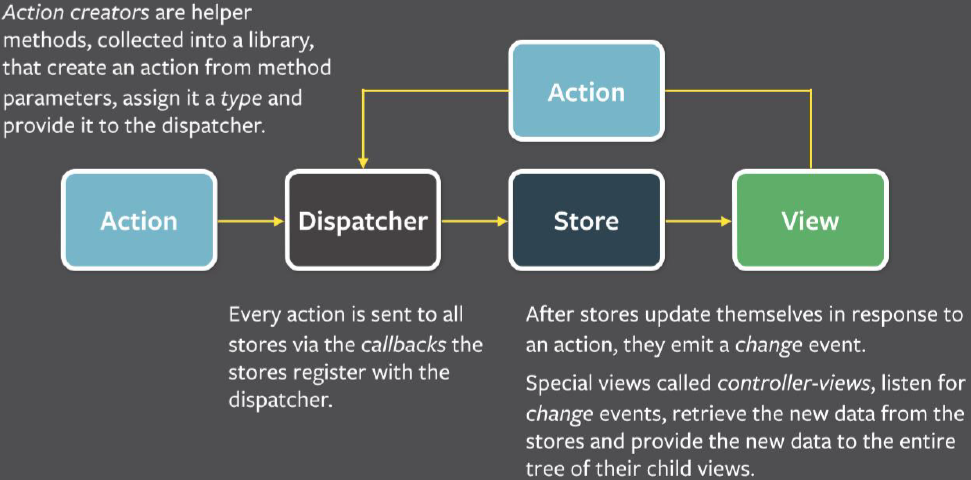
\includegraphics[width=\linewidth]{img/angular_flux_pattern.png}

\subsubsection{Redux Architecture}
\textbf{ngrx:} implements the Redux pattern using RxJS.
\textbf{Benefits:}
\begin{itemize}
    \item Enhanced debugging, testability and maintainability
    \item Undo/redo can be implemented easily
    \item Reduced code in Angular Components
\end{itemize}
\textbf{Liabilities:}
\begin{itemize}
    \item Additional 3rd party library required
    \item More complex architecture
    \item Lower cohesion, global state may contain UI / business data
    \item Data logic may be fragmented into multiple effects/reducers
\end{itemize}

\subsection{UI Advanced}
\subsubsection{Pipes}
Can be applied within a template expression to make small transformations.
\begin{lstlisting}
<p>{{counter.team | uppercase}}</p>
<p>{{counter.team | uppercase | lowercase}}</p>
<p>{{counter.date | date:'longDate'}}</p>
\end{lstlisting}
\textbf{Pure-Pipes:} Executed when it detects a pure change to the input expression.
Implemented as pure functions. Restricted but fast.\\
\textbf{Impure-Pipes:} Executed on every component change detection cycle (every keystroke etc.).
To reduce processing time, caching is often used.\\
\textbf{Predefined-Pipes:} \textit{date, number, currency, async} etc.\\
Angular does not provide Filter- / OrderBy-Pipes because of poor performance.\\
\textbf{Custom-Pipes:} A class decorated with \textit{@Pipe()}.
It implements the PipeTransform interface's \textit{transform()} method.
Needs to be added to the declarations of the current Module.
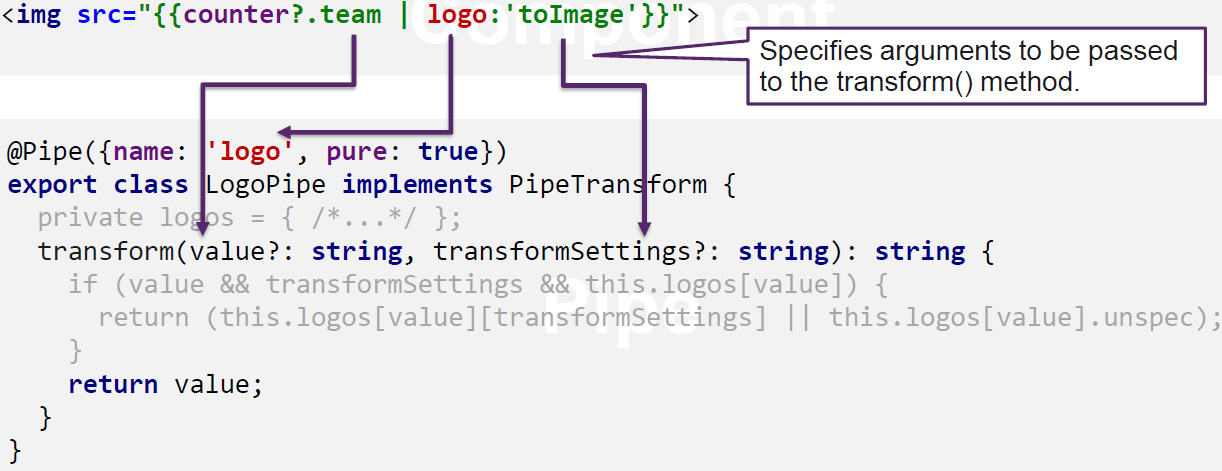
\includegraphics[width=\linewidth]{img/angular_pipes.png}
\textbf{Async Pipes:} Binds Observables directly to the UI.
Changes are automatically tracked.
Automatically subscribes and unsubscribes from the bound Observable.\\
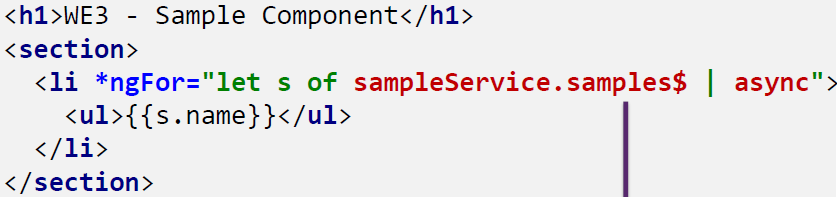
\includegraphics[width=0.6\linewidth]{img/angular_async_pipes.png}
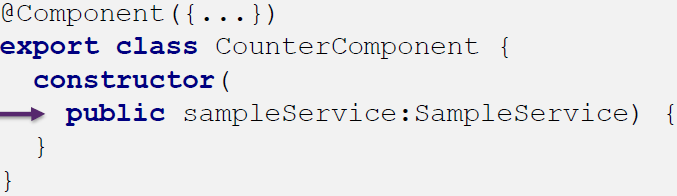
\includegraphics[width=0.4\linewidth]{img/angular_async_pipes2.png}

\subsubsection{View Encapsulation}
\textbf{Component Styles:} Apps are styled with standart CSS.
The CLI transpiles SCSS to CSS.
The selectors of a component's styles apply only within this own template.\\
\textbf{Special Selectors:}
\begin{itemize}
    \item \textit{:host} - Target styles in the element that hosts the component
    \item \textit{:host-context} - Looks for a CSS class in any ancestor of the host element
\end{itemize}
\textbf{Link Styles to Component - Options:}\\
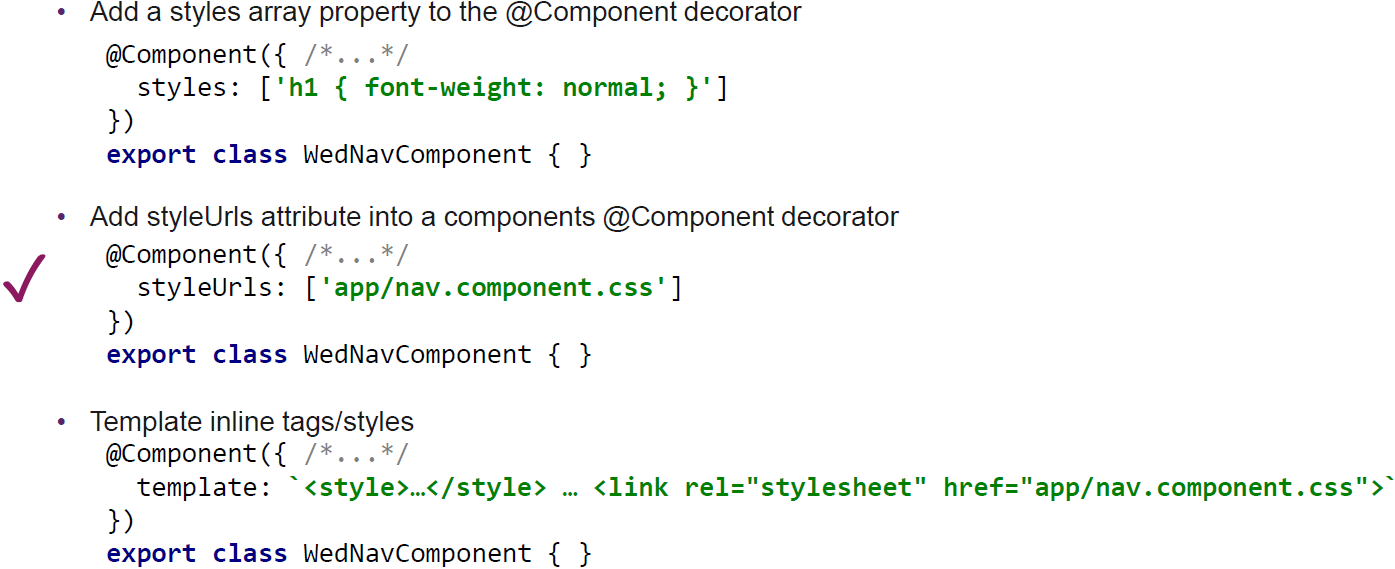
\includegraphics[width=\linewidth]{img/angular_link_styles.png}
\textbf{Controlling View Encapsulation:}
\begin{itemize}
    \item \textit{Native:} Uses the browsers native shadow DOM
    \item \textit{Emulated:} Emulates the behaviour of shadow DOM by preprocessing (and renaming) the CSS
    \item \textit{None:} No view encapsulation (scope rules) applied. All CSS added to the global styles.
\end{itemize}
        %! Author = Philipp Emmenegger
%! Date = 12/07/2021

\section{PWA \& Angular \& Firebase}
\subsection{Angularfire}
\begin{itemize}
    \item Observable based - Use of RxJS, Angular and Firebase
    \item Realtime bindings, synchronized data
    \item Authentication providers
    \item Offline Data
    \item Server-side Render
\end{itemize}

\subsection{PWA}
Progressive Web Apps: Use modern web APIs along with traditional progressive enhancement strategy to create \textbf{cross-platform web apps.}
Work everywhere and have the same user experience advantages as native apps. \textbf{Advantages:} Discoverable, installable, linkable, network independent, progressive, responsive, safe.

\subsection{React - MobX}
\textbf{Straighforward:} write minimalistic, boilerplate free code.
The reactivity system will detect all changes and propagate them out to where they are being used.\\
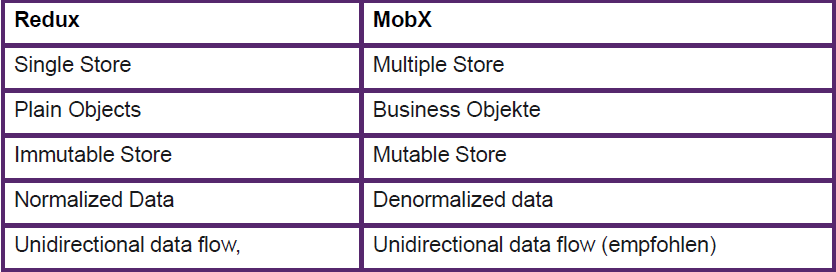
\includegraphics[width=0.6\linewidth]{img/pwa_mobx.png}
        %! Author = Philipp Emmenegger
%! Date = 13/07/2021

\section{ASP.NET CORE}
\textbf{Weshalb:} Enterprise Framework, Kompilierbare Sprache (C\#), Komplett neue Entwicklung, Lauf auf allen Betriebssystemen.
\textbf{Convention over Configuration}.

\subsection{C\#}
\lstset[style=sharpc]
\begin{lstlisting}
// Anonyme Typen
var v =  new { Amount = 100, Message = "Arsch" }
// keine Typechecks / IntelliSense
dynamic person = new ExpandoObject();
// Extesion Methods
public static class MyExtensions {
    public static int WordCount(this string str) {
        return str.Split(new char[] {' ', '.'}).length;
    }
}
\end{lstlisting}

\subsection{Middleware}
\begin{lstlisting}
// Register Middleware
app.Use(async (context, next) => {
    System.Diagnostics.Debug.WriteLine("go req");
    await next.Invoke();
    System.Diagnostics.Debug.WriteLine("end");
});
// Verzweigung für Pfad erzeugen
app.Map("/logging", builder => {
    builder.Run(async (context) => {
        await context.ResponseWriteAsync("Arsch");
    });
});
// Request terminieren, keine neue Middleware
app.Run(async (context) => {
    await context.Response.WriteAsync("Yo");
});
\end{lstlisting}

\subsection{Dependency Injection}
ASP.NET kommt mit einem primitiven DI Container.\\
\textbf{Idee:} Klasse erwähnt welche Interfaces benötigt werden.
Ein Resolver sucht im Container nach einer geeigneten Klasse und übergibt diese.\\
\textbf{DI - Registrierung}
\begin{lstlisting}
public class Startup {
    // called by runtime, Used to add services
    public void ConfigureServices(IserviceCollection services) {
        services.AddTransient<IUserService, UserService>();
    }
    // Called by runtime, Configure HTTP req pipeline
    public void Configure(IApplicationBuilder app, IHostingEnvironment env, ILoggerFactory loggerFactory) {
        app.UseMiddleware<UserMiddleware>();
    }
}
\end{lstlisting}
\textbf{DI - Nutzen}
\begin{lstlisting}
public class UserMiddleware {
    private readonly RequestDelegate _next;
    // Captive Dependency*
    public UserMiddleware(RequestDelegate next, IUserService userService) {
        _next = next;
    }
    // No Captive Dependency
    public async Task Invoke(HttpContext context, IUserService userService) {
        await context.Response.WriteAsync(string.Join(", ", userService.Users));
    }
}
    //
\end{lstlisting}
\subsubsection{Lifetime}
\textbf{Transient:} Created each time they are requested.
Works best for lightweight, stateless services.\\
\textbf{Scoped:} Created once per request.\\
\textbf{Singleton:} Created the first time they are requested.
Every subsequent request will use the same instance.\\
\subsubsection{Captive Dependency}
Komponenten dürfen sich nur Komponenten mit gleicher oder längerer Lebensdauer Injecten lassen.

\subsection{Projekt-Struktur}
\textbf{wwwroot:} Statische Inhalte der Webseite (CSS / JS / HTML).
\textbf{appsettings.json:} Einstellungen der Webseite (Connection-String für DB).
\textbf{Programm.cs:} Einstiegspunkt der WebApp.
\textbf{Startup.cs:} Konfiguriert die WebApp.

\subsection{Razor}
\begin{lstlisting}
@{  var name = "John Doe"; 
    var weekDay = DateTime.Now.DayOfWeek; }
<p>Hello @name, today is @weekDay</p>
\end{lstlisting}

\subsubsection{Wichtige Dateien}
\textbf{Shared/\_layout.cshtml:} Generelles layout der App.
Definiert Sections (Placeholders), welche von der Page gefüllt werden.\\
\textbf{\_Layout.cshtml:} Struktur der Webseite, identisch für jede Seite.
\begin{lstlisting}
@RenderBody() // Platz für Content
@RenderSection("Nav", false); // Platz für Section
@section Nav{ /* ... */ }
\end{lstlisting}
\textbf{\_ViewStart.cshtml:} Hierarchisch, Code welcher vor den Razor-Files ausgeführt wird.
Definiert z.B. das Layout für alle Pages
\begin{lstlisting}
@{ Layout = "_Layout"; }
\end{lstlisting}
\textbf{\_ViewImports.cshtml:} Hierarchisch, Namespaces / Tag-Helpers können in diesem File registriert werden.

\subsubsection{Tag Helpers}
Ermöglichen C\# Code an HTML Tags zu binden.
Bsp: Email-Tag durch Link Tag ersetzen.
\begin{lstlisting}
public class EmailTagHelper : TagHelper {
    public string MailFor { get; set; }
    public override void Process(TagHelperContext context, TagHelperOutput output) {
        output.TagName= "a";
        output.Attributes.SetAttribute("href", "mailto:" + MailFor);
        output.Content.SetContent(MailFor);
    }
}
// Helper im ViewImports-file registrieren
@addTagHelper *, Microsoft.AspNetCore.Mvc.TagHelpers
@addTagHelper *, DataBinding
\end{lstlisting}

\subsubsection{Partials}
Markup Files, verwendet innerhalb von anderen Markup Files. 
Bessere Aufteilbarkeit und Wiederverwendbarkeit.
\begin{lstlisting}
<partial name="_Card" for="Card1" />
<partial name="_Card" model="..." />
\end{lstlisting}

\subsubsection{View Components}
Mächtigere Variante von Partials. 
Beinhalten Logik, können Daten laden / auf bearbeiten.
Rendert ein Teil der Webseite.\\
\textbf{Unterschied zu Pages:} Rendern nur ein Teil der Seite.\\
\textbf{Location:} \textit{/ViewComponents}\\
Razor-File: \textit{Pages/Shared/Components/[ComponentName]/[ViewName]}
\begin{lstlisting}
public class ToDoList: ViewComponent {
    public string[] Todos { get; set; }
    public ToDoList() { /* ... */ }
    public IViewComponentResult Invoke() {
        // /Pages/Shared/Components/TodoList/Default
        return View(Todos);
    }
}
// Razor File
@Page
@{ ViewData["Title"] = "ViewComponent"; }
<vc:to-do-list></vc:to-do-list>
@await Component.InvokeAsync("ToDoList")
\end{lstlisting}

\subsubsection{ViewData / TempData}
Mit Attribut Gekennzeichnete Daten werden allen Razor-Files im Render-Baum übergeben.\\
\textbf{ViewData / ViewBag:} Daten an das \_Layout übergeben\\
\textbf{TempData:} Überlebt ein redirect, Cookie-Middleware nötig (default aktiv)

\subsection{Pages}
Alternative und vereinfachte Variante vom MVC.
Router muss nicht konfiguriert werden.
Best-Practices für Serverseitiges-Rendering.\\
\textbf{Kombination mit MVC:} Statische Seiten mit Pages, REST-API mit MVC.

\subsubsection{Routing}
WebApp generiert anhand der URL eine Antwort.
Bei einem Aufruf wird im Folder \textit{/pages/} nach einer Page gesucht und ausgeführt (\textbf{case insensitive}):\\
\textit{/add} \textrightarrow \textit{/pages/add.cshtml}

\subsubsection{MVVM}
\textbf{*.cshtml:} View mit Razor
\begin{lstlisting}
@page
@model HelloWorldModel
@{ ViewData["Title"] = "HelloWorld"; }
<h1>@Model.HelloWorld</h1>
\end{lstlisting}
\textbf{*.cshtml.cs:} View Model
\begin{lstlisting}
public class HelloWorldModel : PageModel {
    public string HelloWorld { get; set; }
    public void OnGet() {
        HelloWorld = "Hi World!";
    }
}
    //
\end{lstlisting}

\subsubsection{Model}
Pro HTTP-Verb kann im VM eine Funktion definiert werden, die davor aufgerufen wird (OnGet / OnPost etc.).\\
\textbf{Body und Query werden automatisch gemappt:} Parameter werden als Argumente übergeben.
\begin{lstlisting}
public void OnPost(string echoText, long times) {
    EchoText = echoText;
    Times = times;
}
// Param können als Klasse übernommen werden
public void OnPost(EchoModel data) {
    Data = data;
}
// Ohne kopieren der Properties
public class PostModel : PageModel {
    [BindProperty]
    public string EchoText { get; set; }
}
\end{lstlisting}

\subsubsection{View}
\textbf{@page}: Definiert das Razor-File als Page\\
\textbf{@page "/test/\{id?\}":} Überschreibt die Default-Routing-Informationen\\
\textbf{Zugriff auf Routing Parameter:}
\begin{lstlisting}
// Im Razor-File
@page "/test/{id:int?}"
<p>ID: @RouteData.Values["id"]</p>
// Im Model
public int Id { get; set; }
[BindProperty(SupportsGet = true, Name = "Id")]
public int Id2 { get; set; }
public void OnGet(int id) { Id = id; }
\end{lstlisting}

\subsection{AJAX}
\subsubsection{Handlers}
Pages können Actions als handler anbieten.\\
\textbf{Namenskonvention:} \textit{On[Method][Name]}
\begin{lstlisting}
public IActionResult OnPostEcho(strong echoText) {
    return this.Content(echoText);
}
\end{lstlisting}
\textbf{Zugriff:} \textit{[Method]: /[Page]?handler=[HandlerName]}\\
Bsp: POST auf \textit{/Ajax?handler=echo}\\
\textbf{Rückgabewerte (IActionResult)}
\begin{itemize}
    \item ContentResult: StringResult, JsonResult, EmptyResult
    \item Status: NotFoundResult, StatusCodeResult
    \item Redirects: RedirectToPage, RedirectToPagePermanent
    \item Hilfsmethoden: Page(), Partial(), Content()
\end{itemize}

\subsection{Entity Framework}
\textbf{Code First benötigt:} Type Discovery (Welche Klassen in die DB), Connection String, DbContext (Entry Point)\\
\textbf{Migration:} EF Core erlauft keine automatische Migrationen von Model Änderungen mehr.
Aktuell nur über Konsole: \textit{dotnet ef database update}
\subsubsection{Entity Konventionen}
\textbf{public [long/string] Id:} wird automatisch zum PK\\
\textbf{public virtual ApplicationUser Customer:} Als Navigation Property erkannt\\
\textbf{public [long/string] CustomerId:} Als FK für Customer Property erkannt\\
\subsubsection{Wichtige Attribute}
\textbf{[Required]:} NotNull in DB,
\textbf{[NotMapped]:} Nicht in DB geschrieben,
\textbf{[Key]:} Definiert den PK,
\textbf{[MaxLength(10)]:} Allokationsgrösse in DB

\subsection{Validierung}
\subsubsection{Schritt 1: Annotieren der Klassen}
\textbf{Mögliche Attribute:} [StringLength(60, MinimumLength = 3)], [RegularExpression(@"...")], [Required], [DataType(DataType.Date)].
Attribute sind kombinierbar.
\subsubsection{Schritt 2: Razor anpassen}
\textbf{Validation ins DOM einfügen:}
\begin{lstlisting}
<div asp-validation-summary="ModelOnly"></div>
<span asp-validation-for="Item.Name"></span>
\end{lstlisting}
\textbf{JQuery Validation einbinden:}
\begin{lstlisting}
@section Scripts {
    <script src=".../jquery.validate.js"></script>
    <script src=".../...unobtrusive.js"></script>
}
\end{lstlisting}

\subsubsection{Schritt 3: Serverseitige Validierung}
\begin{lstlisting}
[HttpPost]
public ActionResult Index(Order order) {
    if(ModelState.IsValid) {
        order.CustomerId = User.Identity.GetUserId();
        _db.Orders.Add(order);
        _db.SaveChanges();
        return View("OrderOk", order);
    } return BadRequest();
}
\end{lstlisting}

\subsection{Authentifizierung}
\textbf{ASP.NET Identity Features:} PW Stärke, User Validator, Lockout Mechanismus, 2Faktor Auth, Reset PW, OAuth\\
\textbf{ASP.NET Identity Klassen:}
\begin{itemize}
    \item UserManager<ApplicationUser>
    \item RoleManager<IdentityRole>
    \item IAuthorizationService: Validation von Policies
    \item SingInManager
\end{itemize}

\subsubsection{Aktivierung \& Konfiguration}
\textbf{Startup.cs:}
\begin{lstlisting}
services.AddDefaultIdentity<IdentityUser>() // DI
    .AddEntityFrameworkStores<ApplicationDbContext>()
    .AddDefaultTokenProviders();
app.UseIdentity(); // Middleware
// Einstellungen
services.AddDefaultIdentity<IdentityUser>( options => {
    options.Password.RequireDigit = false;
    options.Password.RequiredLength = 8;
}).AddRoles<IdentityRole>()
.AddEntityFrameworkStores<ApplicationDbContext>()
\end{lstlisting}

\subsubsection{Anwenden}
\textbf{Attribute:}\\
\textit{[Authorize]:} User muss authentifiziert sein (Controller/Actions)\\
\textit{[AllowAnonymous]:} Ausnahme für spezifische Action
\begin{lstlisting}
this.User // Eingeloggter User Typ: ClaimsPrincipal
// CRUD Operationen über ApplicationUsers von DI
var user = await _userManager.GetUserAsync(User);
var id = _userManager.GetUserId(User);
\end{lstlisting}
\textbf{Claim:} Statement über einen User, ausgestellt von einem Identity Provider.\\

\subsubsection{Authentifizierung Prüfen}
\begin{lstlisting}
// Automatisch
[Authorize]
public ActionResult Create() { return View(order); }
// Manuell
public ActionResult Create() {
    if(User.Identity.IsAuthenticated) { /* ... */ }
    else { return new StatusCodeResult(401); }
}
\end{lstlisting}

\subsection{Authorisierung}
\begin{lstlisting}
// Lösung 1: Attribute:
[Authorize(Roles = "Admin, PowerUser")]
[Authorize(Policy = "OlderThan18")]
// Lösung 2: Services:
var isInRole =
    await _userManager.IsInRoleAsync(user,"Admin");
// Lösung 3: Claims
User.HasClaim(ClaimTypes.Role, "Admin")
\end{lstlisting}

\subsubsection{Policy}
Ermöglichen es, komplexere Regeln zu definieren.
\begin{lstlisting}
options.AddPolicy("Founders", policy => {
    policy.RequireAuthenticatedUser();
    policy.RequireClaim(ClaimTypes.Name, "joe", "");
});
\end{lstlisting}

\subsubsection{Authorizierung mit Razor}
\begin{lstlisting}
@inject UserManager<ApplicationUser> manager;
@inject ApplicationDbContext context;
@{
    var user = await manager.GetUserAsync(User);
    if(user != null &&
        await manager.IsInRoleAsync(user, "Admin"))
        { /* ... */ }
}
\end{lstlisting}

\subsection{Testing}
\textbf{Unit Test mit ASP.NET}
\begin{lstlisting}
public class UnitTest {
    [Fact]
    public void TestName() { /* ... */ }
}
\end{lstlisting}

\subsection{App Secrets}
Ermöglicht es, Secrets in einem separaten File zu persistieren.
\begin{lstlisting}
// Wert setzen:
dotnet user-secrets set "admin-pwd" "123456"
// Wert nutzen:
if(env.IsDevelopment()) {
    builder.AddUserSecrets<Startup>(); }
app.ApplicationServices.GetService<DataService>()
    .EnsureData(Configuration["admin-pwd"]);
\end{lstlisting}

\subsection{API Routing}
\subsubsection{Startup}
Nur die nötigen Services und Endpoints registrieren.
\begin{lstlisting}
public void ConfigureServices(IServiceCollection services) {
    services.AddRazorPages();
    services.AddControllersWithViews();
    services.AddControllers();
    services.AddMvc();
}
public void Configure(IApplicationBuilder app,
                    IWebHostEnvironment evn) {
    app.UseRouting();
    app.UseEndpoints(endpoints => {
        endpoints.MapControllers();
        endpoints.MapRazorPages();
        endpoints.MapBlazorHub();
    });
}
\end{lstlisting}

\subsubsection{Verwendung}
Funktioniert über Attribute. \textit{[Route]} definiert einen neuen Eintrag im Router.
\textit{[HttpMethod]} bei Actions ist required.\\
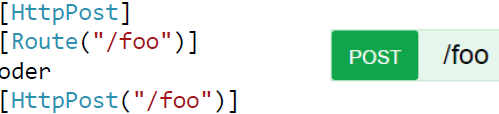
\includegraphics[width=0.45\linewidth]{img/asp_api_routing.png}
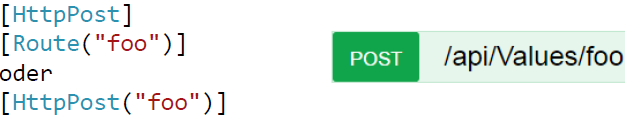
\includegraphics[width=0.55\linewidth]{img/asp_api_routing2.png}

\subsection{Swagger}
Eine Spezifikation für die Dokumentation von REST APIs.
Programmiersprachen unabhängig.
Wird im \textit{Startup.cs} eingetragen.
Defaultmässig unter \textit{http://[server-name]/swagger} erreichbar.
C\# ermöglicht es Kommentare als XML zu exportieren.
Dieses XML-File kann von Swagger genutzt werden um die API zu beschreiben.
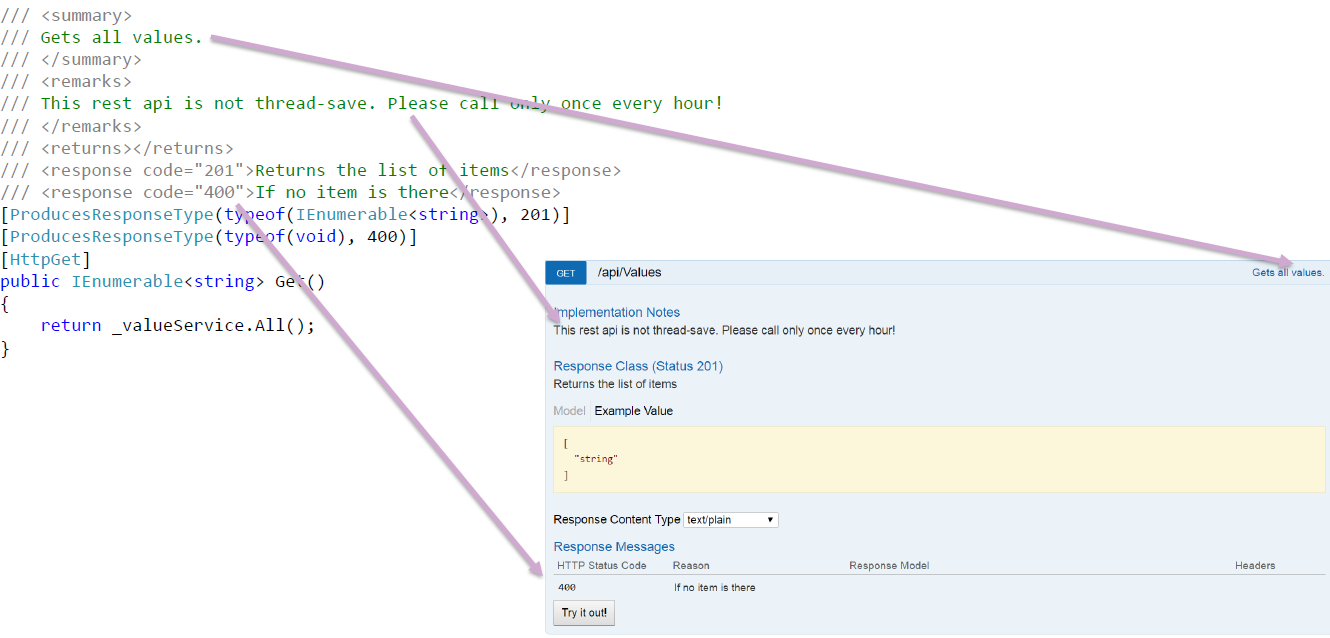
\includegraphics[width=\linewidth]{img/asp_swagger.png}

\subsection{REST HATEOAS}
\textbf{Idee:} Verlinkte Daten als Links zu Verfügung stellen.

\subsection{Exception Handling}
Error Handling soll generisch funktionieren.\\
\textbf{Vorgehen:} Es gibt eine Exception, welche die notwendigen Daten sammelt.
Es gibt einen globalen Errorhandler, welcher diese Exception für Client aufbereitet.
Bei einem ungültigen Zustand wird Custom-Exception ausgelöst.

    \end{multicols*}
\end{document}

























